\subsection{NUMA}
To override the limitations of SMP architecture, the memory can be physically distributed over processors (Fig.~\ref{fig:numa}).
%
With NUMA architecture, latency and bandwidth of each memory access depend on the distance between the processor and the physical locality of the memory.
%
There are several ways to interconnect processors, by connecting all processors together all-to-all the latency can be the lowest possible but once again it's not scalable.
%
It's also possible to connect only some processors together and try to optimize the number of hops like it is done in cluster.
%
At the end, the distance between each NUMA bank can be represented under a matrix form.

%   (-_-)   %
\begin{figure}[!ht]
  \centering
  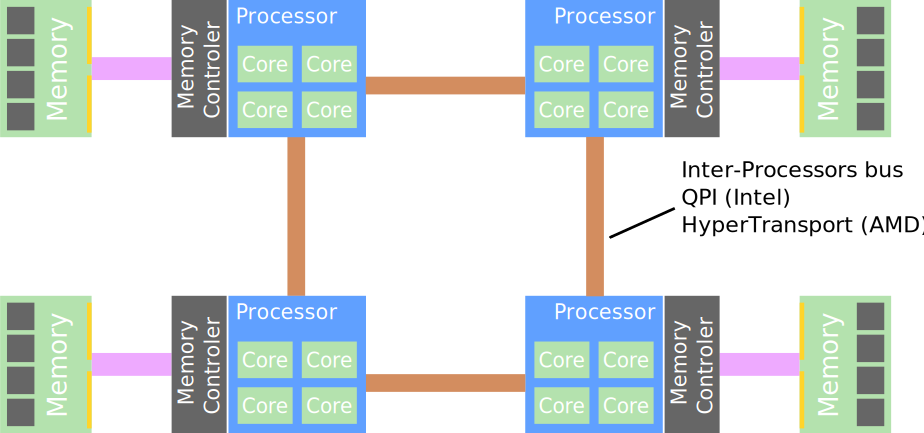
\includegraphics[width=0.8\textwidth]{numa}
  \caption{Overview of an NUMA architecture}
  \label{fig:numa}
\end{figure}
